\documentclass[12pt,a4paper]{article}
\usepackage{ucs}
\usepackage{caption}
\usepackage[latin1,utf8x]{inputenc}
\usepackage{amsmath}
\usepackage{caption}
\captionsetup{font=small,labelfont=bf}
\usepackage[danish]{babel}
\usepackage[rmargin=3cm,tmargin=3.3cm]{geometry}
\usepackage{listings}
\usepackage{color}
\setlength{\parindent}{0pt}
\setlength{\parskip}{1ex plus 0.5ex minus 0.2ex}
\usepackage{graphicx}
\usepackage{fixltx2e}


%insert links
\usepackage{hyperref}
\usepackage{fancyhdr,lastpage}	
\pagestyle{fancy}


\definecolor{mygreen}{rgb}{0,0.6,0}
\definecolor{myblue}{rgb}{0,0,1}
\definecolor{myyellow}{rgb}{0.7,0.7,0}
\definecolor{myblack}{rgb}{0,0,0}

\lstset{
	breaklines=true,
	numbers=left, 
	commentstyle=\color{mygreen},
	stringstyle=\color{myyellow},
}

%header
\lhead{ 
	Embedded Systems \\
	02131 \\ 
}
\chead{ 
}
\rhead{ 2 October, 2012 \\ \bigskip  }

%Footer
\lfoot{
	\rule{\textwidth}{0.1mm}\\
}

\cfoot{}
\rfoot{\ \\ \scriptsize{Side \thepage\ af \pageref{LastPage}}}

\begin{document}

%Forside
\begin{titlepage}
	\begin{center}
		\vspace*{13\baselineskip}
		\huge
		\bfseries
		Embedded Systems\\ 
		\ \\
		02131 \\[5\baselineskip]

		\normalfont
		\Large
		R-peak detection!\\	

		\small
		\vfill
	\end{center}	
	\begin{flushleft}
		Jakob Welner, s124305\\
	 	Jacob Gjerstruo, s113440\\
	\end{flushleft}
\end{titlepage}

\ \\
\section*{Abstract}
The task of this assignment was to develop an Electro-Cardiogram (ECG) scanner using the Pan-Thomkins QRS-Detection Algorithm, and then implement this algorithm in the language C. Using this algorithm, a program has been created that can determine a persons heartbeat, initially using simulated data gathered from an ECG scanner. The conclusion is that it is easily possible to do this, and can recommend the implementation of this algorithm. However, it is desirable to have as many calculations completed through hardware rather than software, as this optimizes the running speed by several magnitudes.

\thispagestyle{empty} 
\newpage

%Table of Contents
\tableofcontents
\thispagestyle{empty} 
\newpage

%Reset pagecount
\setcounter{page}{1}

%Alm. sider
\ \\
\section{Introduction}
	This report will investigate the Pan-Thomas QRS detection algorithm, more specificly, if it is possible to implement this algorithm into the company Medembed's next product, which is a wearable ElectroCardioGram (from now on simply called ECG) scanner.\\
	The algorithm will be implemented in the programming language C, and this report will discuss the following topics: Data acquisition, implementing filters, implementing the peak-detection algorithm, outputting the data to the costumer and finally, an analyzation of the algorithm in terms of power consumption, speed (clock cycles per second) and code size.\\
	For the purpose of this report, we will only implement the C program, and will simulate the data acquisition in real time through data files. Furthermore, the program will be run on an all-purpose processor, whereas in the final product of Medembed, a processor will be designed to do this task.\\
\\
\subsection{Requirements}
Below follows a list of functional and non-functional requirements:\\

\textbf{ Functional requirements for the application:}
\begin{itemize}
	\item Correct data acquisition in simulated real-time
	\item Implementation of the 5 filters
	\item Implementation of the RPeakDetection
	\item Correct output of relevant data to the user, based on the algorithm
	\item An analysis of our implementation, including an analysis of the critical parts, runtime and memory requirements.
\end{itemize}
\textbf{Non-functional requirements for the application:}
\begin {itemize}
	\item The programming language used for this is C
\end{itemize}

\section{Theory}
 	Before we designed the code we were to implement, there were several topics that must be specified first. They are:\\
 	
 	\begin{enumerate}
	\item How should the real-time data acquisition be simulated?
	\item How should the filters be integrated?
	\item How should the RPeakDetection be integrated?
	\item Which data are relevant for the user, and how should it be shown?
	\item How do you determine the critical parts?
\end{enumerate}

\subsection{Problem 1: Data acquisition}
	As specified in the introduction, the dataset used is simulated and not a real patient. To ensure the capability of the program, and to ease the transition to hardware-coding, a requirement was that the whole dataset must not be loaded into one array - instead, it must be loaded one data-point at a time. This introduces a few challenges, the biggest being how to ensure that the entire dataset is processed, no matter the size.\\

\subsection{Problem 2: Implementation of Filters}
	To use the QRS-algorithm, the dataset must first be run through 5 filters, each of which must be implemented. Of these filters, 4 of them requires both the current data point, but also previous data points. This creates two challenges - one being how to ensure that the program does not encounter data under- and overflow, and the other being how the data points are to be transferred from the program to the filters.\\
\\	
	To the first of these challenges, the easiest way to do this would be to implement the filters with strict if/else sentences. Alternatively, when the index reaches the first negative value, one could add the size of the array and have the index moving backwards through the end of the array of the dataset currently used.\\
	To the second of these challenges, there are two solutions: Either, two arrays, x and y, could be used. Here, x will hold the data would operate on and y will hold the data that has already been filtered. Alternatively, a struct could be created.\\

\subsection{Problem 3: Implementation of RPeakDetection}
	Once all the filters has been implemented, the actual QRS-algorithm has to be implemented. This QRS-algorithm will be the one that determines what consitutes a heartbeat, and how to analyse this heartbeat. Furthermore, it will determine what is a peak and what is not, and after each peak, it will update certain variables to ensure the heartbeats are tracked correctly. These variables will be the ones determining when a heartbeat is certain than a threshold, and if it is, this peak is referred to as an R-peak. Once an R-peak has been determined, data is updated further to classify the next peaks as either heartbeats or noise. This algorithm, however, introduces two challenges - how to determine whether the patient simply has irregular and/or weak heartbeaks or whether the patient is having a heart attack; and how to ensure that every heartbeat is detected correctly.\\
	\\

\subsection{Problem 4: Relevant data}
	The requirement states that the program must show at the very least the value of the latest R-peak that was detected, and also, it must show when this R-peak happened, plus the patients pulse. Furthermore, the patient must be given a warning of the R-peaks value is less than 2000 (as this is a sign of an impending heart attack) and finally, if 5 successive RR-intervals has missed the RR- LOW and HIGH values, these must be shown. However, how these data are to be shown has not been defined, and therefore must be specified.\\
	\\
	There are several ways to show these data, of which the simplest is to make a text-based screen with the information necessary, and keep this screen updated in real-time, showing the data as we calculate them. Alternatively, the data can be plotted and shown in a graph, or one could combine these two, giving both a graph that keeps getting updated in real-time, as well as text-based information.\\

\subsection{Problem 5: Critical parts}
	The final issue that was to be clarified is the critical parts of the program. Here, there are three points to discuss, memory requirement, time consumption and power consumption.\\
	Memory requirement is important as the bigger the program is, that is, the more memory it requires, the more physical memory must be implemented into the final device, and therefore, the device will become larger and more cumbersome to wear. Furthermore, more memory also means that the device becomes more power-consuming.\\
	Time consumption is important as the device must be able to read at least 250 data points a second, and if the functions are very time consuming, a stronger processor is needed that requires more power. Furthermore, it is also important that the processor used does not process the data too fast, either, as this will mean that the processor will idle and use power for nothing, meaning a smaller processor can be used that requires less power.\\
	Power consumption is important as it determines how often the user must either recharge the battery or be issued a new battery.\\
	
\section{Design}
	When designing the program, it was quickly decided that multiple files should be used for easier readability. Each file would consist of functions native to the file (for instance, the filter.c would contain filters only). The files used are: filter.c, buffer.c, main.c, RRhandling.c, sensor.c, peakDetect.c.\\
	\\
	Furthermore, it was decided that the data from each filter, as well as the raw data, would each be stored in an array of up to 50 data points - having more than this would be a waste of memory, and having less than this presented the risk of not having enough data points for the filters.\\
	\\
	To load the actual data into the arrays, a buffer was created in combination with a loop. The loop would run through the data-set, scanning in a point and then passing it to the buffer. The buffer would then store this data point in the correct array, and this array would then be passed on to the filters. Once the filters calculate the correct value, the value would be returned to the buffer that would store this in the correct place in the array.\\
	The buffer will also keep track of where in the array the data is, and should it exceed the size of the array, it will return to the first place in the array (indexed to 0) and overwrite the data there.\\
	\\
	%write something about R-peak detection design decisions


\section{Implementation}
\subsection{Real-time data acquisition}
	As described, the program must acquire the data and calculate in real-time. To ensure this simulation, the program loads one data point, then passes it and the corresponding array to the one filter at a time before it finally passes it to the peak detection and subsequently, to the R-peak detection. Once all these calculations have been done, it loads in a new data point and restarts through a while loop.\\
	This while-loop will run through the entire data-set, and will not stop before it reaches the end of the file (in the finished product, it will of course run until the battery runs dry).\\
	\\
	Therefore, the combination of the while-loop that runs forever, and the continual loading and subsequent calculations solves the challenge of real-time data acquisition.\\

\subsection{Implementation of Filters}
	The first implementation of the filters were simply done with strict if/else sentences. However, this was changed to using an adaptive index that, should it reach negative values, moves to the end of the array instead. This way, the program should never encounter data under- or overflow, and thereby, the first of the challenges were solved.\\
	The second challenge, to ensure the correct transfer of data from one filter to another, was solved by using two arrays, one for the raw data and one for the filtered data. Each array is then passed to the next part of the program, ensuring all filters have both raw and processed data to be operated on, as 4 of them requires.\\
	\\
	Therefore, the use of two arrays and an adaptive index solves the challenge of the implementation of the filters.\\
	
\subsection{Implementation of RPeakDetection}
	
\subsection{Relevant data}
	To display the relevant data, a simple text-based display was created. This would show the required information, that is, the value of the latest R-peak, the time of the R-peak, the patients pulse. Furthermore, it will also display the warning and the RR-LOW and RR-HIGH values if 5 RR-intervals has been missed.\\
	\\
	Therefore, the challenge of the relevant data has been solved.
\subsection{Critical parts}

\begin{figure}[h!]
%  \centering
%   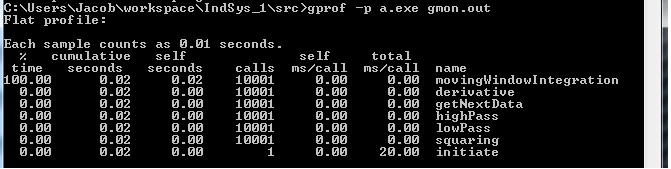
\includegraphics[width=1\textwidth]{results_time.png}
%  \caption{The table above shows the time spent in the various filters in our program}
\end{figure}

\section{Results}
\subsection{Testresults of filters}

\begin{figure}[h!]
%  \centering
%    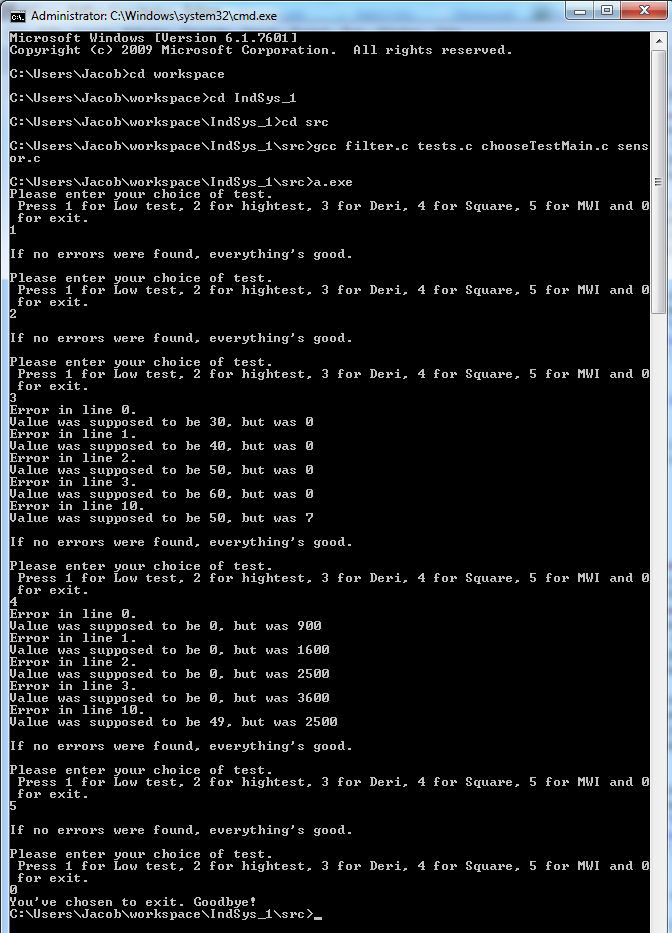
\includegraphics[width=0.5\textwidth]{Results_test.png}
%  \caption{The results of our test cases of the 5 filters.}
\end{figure}
\subsection{Testresults of RPeakDetection}

\section{Discussion}
% Could be very interesting to have a discussion here about what we put in software / hardware, i.e. what we put in software is what we think will change the most. Furthermore, could be %interesting to discuss the technical fremskridt, like kinetic energy transformed into power through walking.
%Discussion on when to use searchback

\section{Conclussion}

\newpage
\begin{thebibliography}{9}

\bibitem{lamport94}
  Michael Reibel Boesen, Linas Kaminskas, Paul Pop, Karsten Juul Frederiksen\\
  \emph{Assignment 1: Software implementation of a personal ECG scanner}\\
  3rd Edition\\
  2013.

\bibitem{power consumption}
	http://www.notebookcheck.net/Intel-Core-i7-2630QM-Notebook-Processor.41483.0.html\\
	Date of use: 25/09/2013
\end{thebibliography}
	
\newpage	
	\begin{Large}
		\textbf{Appendix}
	\end{Large}
	\appendix

\section{Who wrote what}
Jacob Gjerstrup, s113440 wrote: \\
Jakob Welner, s124305 wrote: \\
	
\section{Sourcecode - introductionary exercises}
\subsection{ReadFromFile}
	Below is the sourcecode for the introductionary-exercise (From september the 4th) - more precisely, the ReadFromFile source-code.\\
	\\
	\lstinputlisting[language=C]{Code/Exercise/main.c}

\subsection{HelloWorld}
	The next is the sourcecode from the same exercise - this time, it's the sourcecode of our HelloWorld program.\\
	\\
	\lstinputlisting{Code/Exercise/HelloWorld.c}
	
\section{Sourcecode - the real program}
	Below follows the sourcecode for each of the parts of our program, split into sections. The first part, the program, is where the various functions are called, and all our data is stored. The Filter.c contains the 5 different filters. The RPeakDetection contains the detection of each peak, along with the calculations of the various thresholds. The sensor is what scans data from the file, and thus simulates that we scan the patient, and finally, the header files is what contains all the prototypes for our functions.
\subsection{Buffer}
	\lstinputlisting[language=C]{Code/buffer.c}	
\subsection{Filters}
	\lstinputlisting[language=C]{Code/filter.c}
\subsection{RPeakDetection}
	R-Peak detection consists of two files - peak detection and RR Handling.\\
	Peak detection:\\
	\lstinputlisting[language=C]{Code/peakDetect.c}	
	RR Handling:\\
	\lstinputlisting[language=C]{Code/RRhandling.c}	
\subsection{Sensor}
	\lstinputlisting[language=C]{Code/sensor.c}	
\subsection{Header files}
\subsubsection{sensor.h}
	Below is the first of the header files, called sensor.h. This file contains the prototype for the sensor as well as the peak detection.\\
	\lstinputlisting{Code/sensor.h}
\subsubsection{buffer.h}
	After this one, the next header file called filter.h comes - this file contains the prototypes of the filters as well as for the buffer.\\
	\lstinputlisting{Code/buffer.h}
\subsection{Tests}
%	We decided to do a run of tests, as discussed in the report. Below is the sourcecode for the tests:
\subsection{Tests of RPeakDetection}
%	\lstinputlisting{RPeakTest.c}
\subsubsection{tests}
%	\lstinputlisting{tests.c}
\subsubsection{Main function for test cases}
%	\lstinputlisting{chooseTestMain.c}
\end{document}